Uma das características das plataformas que suportam simulações físicas como o Chipmunk é a capacidade de detectar colisões entre os objetos. 
Para detectar colisões de forma eficiente essas plataformas utilizam um processo com duas fases: \textit{broad phase} e a \textit{narrow phase}.\\

A finalidade da \textit{broad phase} é evitar a realização de cálculos caros para corpos distantes um dos outros. Para
gerar os pares de objetos que devem passar pelo algoritmo de detecção de colisão, o Chipmunk suporta as seguintes estruturas de dados:
árvores AABB e o \textit{spatial hashing}. Na versão 5 do Chipmunk a estrutura de dados utilizada é o \textit{spatial hashing} enquanto na versão 6 são as árvores AABB. \\

\textit{Narrow phase} é a fase onde pares de objetos são verificados cuidadosamente em termos de colisão. O Chipmunk utiliza nesta fase o \textit{Separating Axis Theorem}, que suporta somente polígonos convexos. Devido a esse motivo, não é possível criar objetos côncavos no Chipmunk. \\

Nas próximas seções serão explicadas resumidamente os algoritmos de cada fase.

\subsection{\textit{Broad phase} - Árvore AABB}

Para entender a árvore AABB, é preciso primeiro entender o que é AABB. AABB é um acrônimo para \textit{Axis Aligned Bounding Box}, ou seja, caixas delimitadoras de objetos 
em formas de retângulo alinhadas com os eixos x e y, como mostra a figura \ref{mariobb}:

\begin{figure}[!htbp]
  \centering
  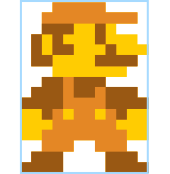
\includegraphics[scale=0.3]{mario_bb.png} 
  \caption{O retângulo azul representa uma caixa delimitadora do objeto \protect\cite{mario:bb}.}
  \label{mariobb}
\end{figure}

A árvore AABB é uma árvore binária que faz proveito da estrutura da AABB para armazenar e consultar objetos no espaço 2D. O nó da árvore pode guardar o próprio objeto 
ou possuir dois nós filhos. Quando um nó guarda um objeto, a caixa delimitadora deste nó deve conter a caixa delimitadora do objeto. Se o nó possui nós filhos, 
sua caixa delimitadora deve conter as caixas delimitadoras dos nós filhos. 
Um ponto importante é que esta estrutura precisa de uma heurística para inserir os nós na árvore. No caso do Chipmunk existe uma heurística baseada na caixa 
delimitadora do objeto e também em relação à sua velocidade. Na figura \ref{aabb} mostramos um exemplo de uma árvore AABB de três objetos A, B e C: 

\begin{figure}[!htbp]
  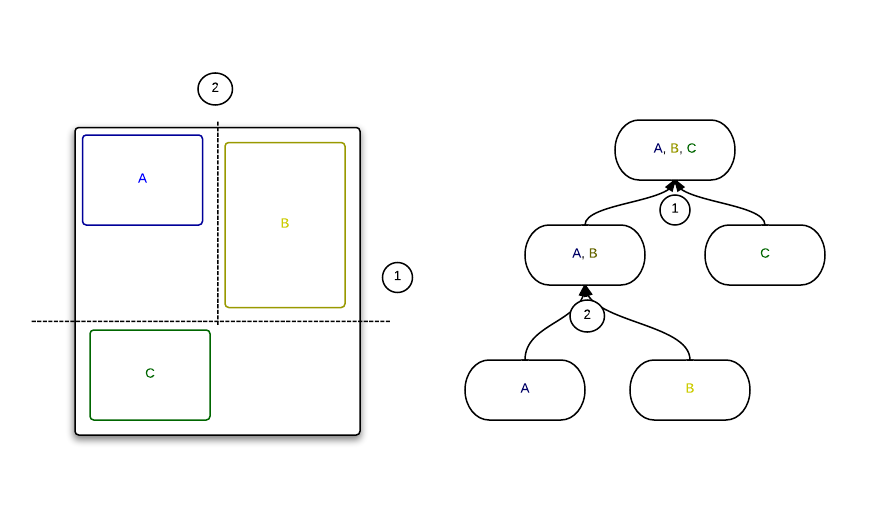
\includegraphics[scale=0.4]{AABBTree.png}
  \caption{Exemplo de uma árvore AABB}
  \label{aabb}
\end{figure}

A caixa delimitadora da raiz é o retângulo preto contendo os objetos A, B e C.
As duas novas caixas delimitadoras criadas pela linha indicado pelo número 1 são agora filhas da raiz. 
E finalmente a linha indicado pelo número 2 criam mais duas caixas delimitadoras separando os objetos A e B.\\

A figura \ref{aabbTree} mostra como são definidos os pares de objetos que passarão pela \textit{narrow phase}. Começando pela raiz, a caixa delimitadora do objeto D intersecta somente 
com a caixa delimitadora do nó esquerdo. Em seguida, a caixa delimitadora do objeto D intersecta somente com a caixa delimitadora da folha contendo o objeto A.
Então o par criado nessa busca é o par \{A, D\}.

\begin{figure}[H]
  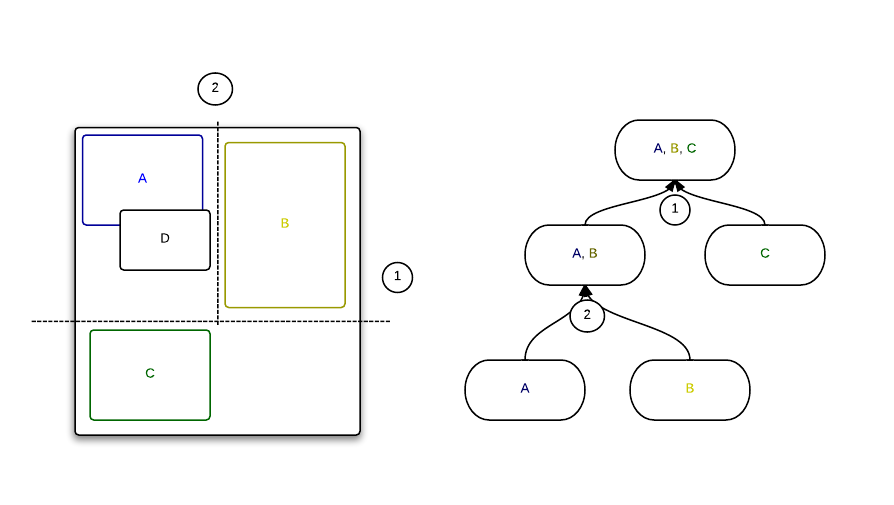
\includegraphics[scale=0.4]{AABBTree1.png}
  \caption{Exemplo de detecção de colisão. O objeto D é comparado somente com a folha contendo o objeto A.}
  \label{aabbTree}
\end{figure}

\subsection{\textit{Broad phase} - 1D \textit{sweep and prune}}

A idéia deste algoritmo é varrer as caixas delimitadoras dos objetos criando assim os pares de objetos que deverão ser passados para a fase seguinte. \\

Seguindo o exemplo da figura \ref{sweep}, o algoritmo mantém uma lista de objetos que estão sendo varridos. Quando a varredura encontra o início do objeto, ela o inclui na lista. 
Quando a varredura encontra o final do objeto, ela o exclui da lista. No exemplo observamos que a lista [A, B, C] criam os pares \{A, B\}, \{A, C\} e \{B, C\} 
enquanto a lista [B, D] cria o par \{B, D\}. \\

\begin{figure}[!htbp]
  \centering
  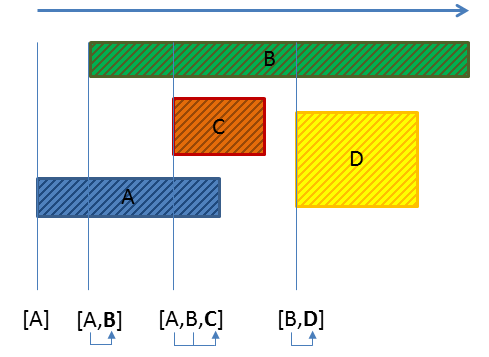
\includegraphics[scale=0.7]{sp.png}
  \caption{Exemplo de funcionamento do algoritmo \textit{sweep and prune} \protect\cite{broad:sweep}}
  \label{sweep}
\end{figure}

Esse algoritmo, de acordo com a documentação do Chipmunk 6, pode ser muito eficiente em jogos voltados para dispositivos móveis se o seu mundo é muito comprido 
e plano como um jogo de corrida.

\subsection{\textit{Broad phase} - \textit{Spatial hashing}}

\textit{Spatial hashing} é um processo onde o espaço de duas ou três dimensões é projetado em uma tabela \textit{hash} de uma dimensão. Para isso o Chipmunk divide o espaço em 
células do mesmo tamanho, onde cada célula é mapeada a uma entrada na tabela \textit{hash}. Um objeto sempre é mapeado nas células que ele está presente. Com esta estrutura 
  é fácil de criar os pares de objetos. Dado um objeto precisamos verificar quais as células que ele está presente e criar o par para cada objeto existente nas 
entradas da tabela destas células.\\

O tamanho das células é de suma importância para obter uma boa eficiência. Nas próximas figuras, as áreas cinzas representam as células. Quanto mais escuras, mais objetos estão mapeadas na célula. O ideal é que o tamanho das células não seja muito pequeno nem muito grande.\\

\begin{figure}[!htbp]
  \centering
  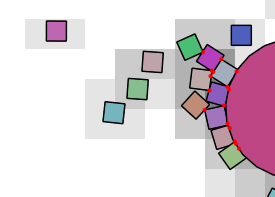
\includegraphics[scale=1]{hash_just_right.png}
  \caption{Cada célula contém poucos objetos. Estado ideal para \textit{spatial hashing} \protect\cite{Chipmunk:image1}}
\end{figure}

\begin{figure}[!htbp]
  \centering
  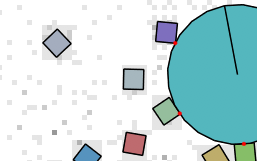
\includegraphics[scale=1]{hash_too_small.png}
  \caption{Cada objeto está mapeado em muitas células \protect\cite{Chipmunk:image2}}
\end{figure}

\begin{figure}[!htbp]
  \centering
  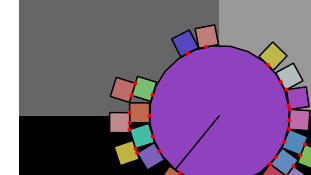
\includegraphics[scale=1]{hash_too_big.png}
\caption{Cada célula contém muito objetos \protect\cite{Chipmunk:image3}}
\end{figure}

Esta estrutura de dados é a mais indicada quando a simulação possui um conjunto grande de objetos e de mesmo tamanho.

\subsection{\textit{Narrow phase} - \textit{Separating Axis Theorem}}

No Chipmunk existe somente um algoritmo para detecção de colisão, baseado no \textit{Separating Axis Theorem}. A idéia do algoritmo é verificar se é possível desenhar um segmento 
de reta entre duas formas convexas. Se existe tal segmento, então não há colisão entre eles, caso contrário, as duas formas estão colidindo. No caso de formas
côncavas isso não é verdade. Devido a essa restrição do algoritmo o Chipmunk impõe que todo polígono seja convexo. \\

É um algoritmo rápido que elimina a necessidade de ter um código de detecção de colisão para cada tipo de forma. A figura \ref{narrow} ilustra a idéia do algoritmo.

\begin{figure}[!htbp]
  \centering
  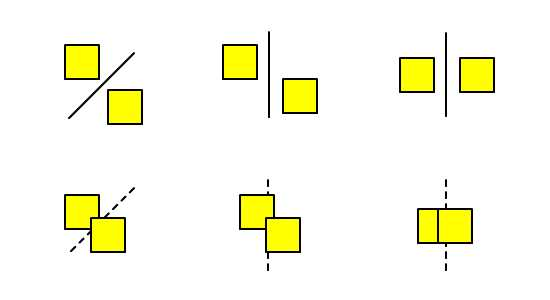
\includegraphics[scale=0.5]{SAT.jpg}
  \caption{Se existe uma linha que separa os polígonos convexos, então eles não estão colidindo \protect\cite{narrow:sat}.}
  \label{narrow}
\end{figure}
